% !TEX program = xelatex
\RequirePackage{expl3}
\ExplSyntaxOn
\cs_if_exist:NF \prop_gput_if_not_in:Nnn {
  \cs_gset_eq:NN \prop_gput_if_not_in:Nnn \prop_gput_if_new:Nnn
}
\ExplSyntaxOff

%%%%%%%%%%%%%%%%%%%%%%%%%%%%%%%%%%%%%%%
% PlushCV - One Page Two Column Resume
% LaTeX Template
% Version 1.0 (11/28/2021)
%
% Author:
% Shubham Mazumder (http://mazumder.me)
%
% Hacked together from:
% https://github.com/deedydas/Deedy-Resume
%
% IMPORTANT: THIS TEMPLATE NEEDS TO BE COMPILED WITH XeLaTeX
%
% 
%%%%%%%%%%%%%%%%%%%%%%%%%%%%%%%%%%%%%%
% 
% TODO:
% 1. Figure out a smoother way for the document to flow onto the next page.
% 3. Add more icon options 
% 4. Fix hacky left alignment on contact line
% 5. Remove Hacky fix for awkward extra vertical space
% 
%%%%%%%%%%%%%%%%%%%%%%%%%%%%%%%%%%%%%%
%
% CHANGELOG:
%
%%%%%%%%%%%%%%%%%%%%%%%%%%%%%%%%%%%%%%%
%
% Known Issues:
% 1. Overflows onto second page if any column's contents are more than the vertical limit.
%%%%%%%%%%%%%%%%%%%%%%%%%%%%%%%%%%%%%%
%%Icons:
%%Main: https://icons8.com/icons/carbon-copy
%%%%%%%%%%%%%%%%%%%%%%%%%%%%%%%%%%

\documentclass[]{plushcv}
\usepackage{fancyhdr}
\usepackage{tikz}
\pagestyle{fancy}
\fancyhf{}
\hyphenpenalty=10000

\begin{document}

%%%%%%%%%%%%%%%%%%%%%%%%%%%%%%%%%%%%%%
%
%     TITLE NAME
%
%%%%%%%%%%%%%%%%%%%%%%%%%%%%%%%%%%%%%%
\vspace*{1mm}
\noindent\begin{minipage}[t]{0.17\textwidth}
  \vspace{0pt}
  \begin{tikzpicture}
    \clip (0,0) circle (1.5cm);
    \node at (0,-0.2) {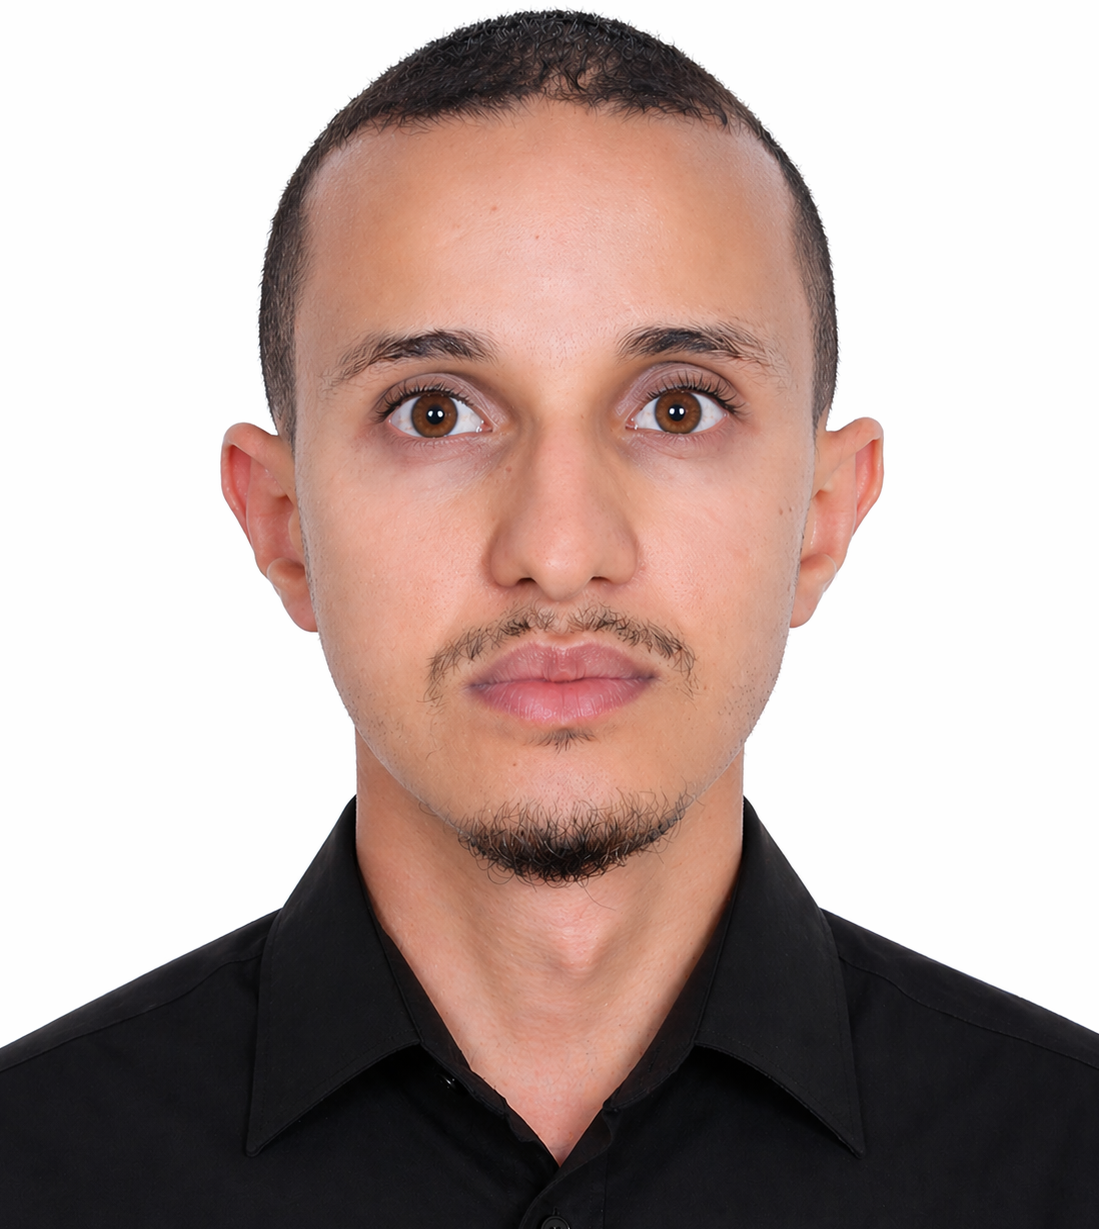
\includegraphics[width=3.2cm]{assets/imageee.png}};
  \end{tikzpicture}
\end{minipage}%
\hspace{0.05cm}
\begin{minipage}[t]{0.78\textwidth}
\namesection{Izelmadene}{Achraf}
{  \normalsize Futur Ingénieur en Génie Électrique et Systèmes Intelligents}
%Futur Ingénieur
{\contactline{\href{https://www.linkedin.com/in/achraf-izelmadene/}
{ACHRAF IZELMADENE}}
{\href{mailto:achraf.izelmadene@gmail.com}
{achraf.izelmadene@gmail.com}}
{\href{tel:+212699098736}
{+212699098736}}}
\end{minipage}
\vspace{0.1em}
\begin{minipage}[t]{0.72\textwidth} 


%%%%%%%%%%%%%%%%%%%%%%%%%%%%%%%%%%%%%%
%     À propos
%%%%%%%%%%%%%%%%%%%%%%%%%%%%%%%%%%%%%%

\section{À propos}
Élève Ingénieur en Génie Électrique et Systèmes Intelligents (GESI), spécialisé en efficacité énergétique et digitalisation industrielle. Fort d'une expérience terrain en milieu industriel et d'une expertise en Data Science (Python, Machine Learning), je recherche un PFE de Responsable Projet Énergie. Je souhaite mettre à profit mes compétences en création de tableaux de bord, analyse de données et systèmes énergétiques pour optimiser la performance et réduire les émissions CO2 de vos clients.
\sectionsep
%\vspace{5mm}
\section{Education}
\runsubsection{Diplôme d'ingénieur en Électrique et Systèmes Intelligents}
\descript{École Marocaine des Sciences de l'Ingénieur \textbf{(EMSI)}}\hfill\location{2025 - Présent}\\
\hspace{1em}{\color{headings}\fontsize{7.5pt}{10pt}\selectfont \textbf{Cours :} \textit{Automatique \& Régulation \textbullet{} Systèmes Embarqués \textbullet{} Capteurs \& Actionneurs \textbullet{} Maintenance Industrielle \textbullet{} Robotique \textbullet{} Réseaux et Sécurité Électrique \textbullet{} Gestion de Projet}}
\sectionsep
\\
\runsubsection{Licence en Sciences de la Mati\`ere Physique  \space \small\textit{Option: Automatique}} {}
%fondamentale
\descript{Faculté des Sciences Semlalia de Marrakech \textbf{(FSSM)}}\hfill\location{2020-2024}\\
\hspace{1em}{\color{headings}\fontsize{7.5pt}{10pt}\selectfont \textbf{Cours :} \textit{Électricité \& Électronique \textbullet{} Automatisme \& Asservissements \textbullet{} Thermodynamique \textbullet{} Mécanique Générale \textbullet{} Informatique C++}}
\sectionsep
\\
\runsubsection{Baccalauréat Sciences Physiques (PC)}
\descript{ Lycée Al Maghrib Al Arabi Marrakech}\hfill\location{2020}
\sectionsep
%%%%%%%%%%%%%%%%%%%%%%%%%%%%%%%%%%%%%%
%     Experience
%%%%%%%%%%%%%%%%%%%%%%%%%%%%%%%%%%%%%
\section{Experience}
\runsubsection{Stagiaire en unité de production }
\descript{Ménara Préfa}\hfill\location{ JUL 2024}
\vspace{\topsep} %% JUST LET THIS HERE 
\begin{tightemize}
\item Migration d'un automate vers un Siemens S7 ; suivi des opérations et mise à jour de documents techniques.
\item Sensibilisation aux procédures de maintenance préventive et corrective sur lignes de production.
\end{tightemize}
\vspace{\topsep}
\runsubsection{Stagiaire en Bureau d'Études}
\descript{CORE ENGINEERING SOLUTIONS}\hfill\location{JUL -- AOÛT 2026}
\vspace{\topsep}
\begin{tightemize}
\item Dimensionnement d'un poste de livraison HTA/BT et étude d'intégration solaire en autoconsommation pour une zone industrielle (AutoCAD, Caneco BT, PVsyst).
\item Réalisation de schémas unifilaires, bilans de puissance et notes de calculs détaillées.
\end{tightemize}

\section{Projets}

\runsubsection{Smart Agriculture IoT Ecosystem}
\vspace{1pt}
\begin{tightemize}
\item Collection de données IoT via réseau de capteurs (Arduino, ESP32, modules LoRa) et création de tableaux de bord interactifs pour le suivi en temps réel et la prise de décision.
\end{tightemize}
\vspace{1pt}
\runsubsection{Analyse Énergétique Smartgrid (Data Science \& Machine Learning)}
\vspace{1pt}
\begin{tightemize}
\item Modèles de clustering (KMeans, DBSCAN, GMM) sur données de consommation électrique ; élaboration de tableaux de bord pour analyser les dérives énergétiques.
\end{tightemize}
\vspace{1pt}
\runsubsection{Maintenance Prédictive Industrielle (AutoML)}
\vspace{1pt}
\begin{tightemize}
\item Analyse de la cohérence des données industrielles et comparaison de modèles de Machine Learning (TPOT vs Auto-WEKA) pour anticiper les défaillances et configurer des alarmes.
\end{tightemize}
\vspace{1pt}

\vspace{-3pt}

%%%%%%%%%%%%%%%%%%%%%%%%%%%%%%%%%%%%%%
%
%     COLUMN TWO
%
%%%%%%%%%%%%%%%%%%%%%%%%%%%%%%%%%%%%%%

\end{minipage} 
\hfill
\begin{minipage}[t]{0.24\textwidth} 

%%%%%%%%%%%%%%%%%%%%%%%%%%%%%%%%%%%%%%
%     SKILLS
%%%%%%%%%%%%%%%%%%%%%%%%%%%%%%%%%%%%%%
\section{Skills}
\sectionsep
\vspace{2pt}

\subsection{Programming}
\sectionsep
C/C++ \textbullet{} Python \textbullet{}\\ JavaScript \textbullet{} HTML/CSS
\sectionsep
\vspace{2pt}

\subsection{LOGICIELS}
\sectionsep
AutoCAD \textbullet{} Caneco BT \textbullet{} PVsyst \textbullet{} \\
Dialux EVO \textbullet{} MATLAB \textbullet{} TIA PORTAL \textbullet{} 
SolidWorks \textbullet{} TinkerCAD  \textbullet{} 
Pack Office \\(Word, Excel, PowerPoint)
\vspace{2pt}

\sectionsep
\subsection{Tools/Platforms}
\sectionsep
Git \textbullet{} Docker \textbullet{} PyBullet \\
Arduino \textbullet{} Supabase \textbullet{}\\ 3DEXPERIENCE \\
\sectionsep
\vspace{2pt}
\subsection{Divers}
\sectionsep
Permis de conduire B\\

%%%%%%%%%%%%%%%%%%%%%%%%%%%%%%%%%%%%%%
%     EDUCATION
%%%%%%%%%%%%%%%%%%%%%%%%%%%%%%%%%%%%%%
\vspace{4pt}
\section{CERTIFICATIONS}
\sectionsep

\subsection{3DEXPERIENCE Collaborative \\ Industry Innovator}
\descript{Dassault Systèmes}
\vspace*{2pt}

\subsection{Sensors and Sensor Circuit Design}
\descript{Univ. of Colorado Boulder | Coursera}
\vspace*{2pt}

\subsection{Machine Learning in Production}
\descript{DeepLearning.AI | Coursera}
\vspace*{2pt}

\subsection{Foundations of IoT Systems}
\descript{LearnQuest | Coursera}
\sectionsep
\vspace{2pt}
\section{Awards}
\begin{tabular}{@{}p{0.5cm} p{3.8cm}}
\textbf{\large 1st} & \textbf{Hack The Intelligence} \\
 & {\footnotesize AISEC Int'l Summit \textbf{2026}} \\[4pt]
\textbf{\large 2nd} & \textbf{Vision AI Competition} \\
 & {\footnotesize EMSI Marrakech \textbf{2026}} \\
\end{tabular}
\vspace{-2pt}
\section{Langues \& Divers}
\vspace{0pt}

\begin{flushleft}
Arabe (maternelle) \textbullet{} Français (DELF B2) \textbullet{} Anglais (EFSET B2)
\end{flushleft}

\end{minipage} 
\end{document}
